
%%%%%%%%%%%%%%%%%%%%%%%%%%%%%%%%%%%%%%%%%%%%%%%%%%%%
%    Jordan Scott    %
%%%%%%%%%%%%%%%%%%%%%%%%%%%%%%%%%%%%%%%%%%%%%%%%%%%%
%\documentclass{article}

%\usepackage[utf8]{inputenc}
%\usepackage[english]{babel}
%\usepackage{graphicx}


%\begin{document}
	
	%\title{CS6000 Journal}
	%\author{Jordan Scott} 
	%\maketitle
	
	\section{\textbf{CS6000 Journal - Jordan Scott}}
	
	
	\begin{figure}
		\centering
		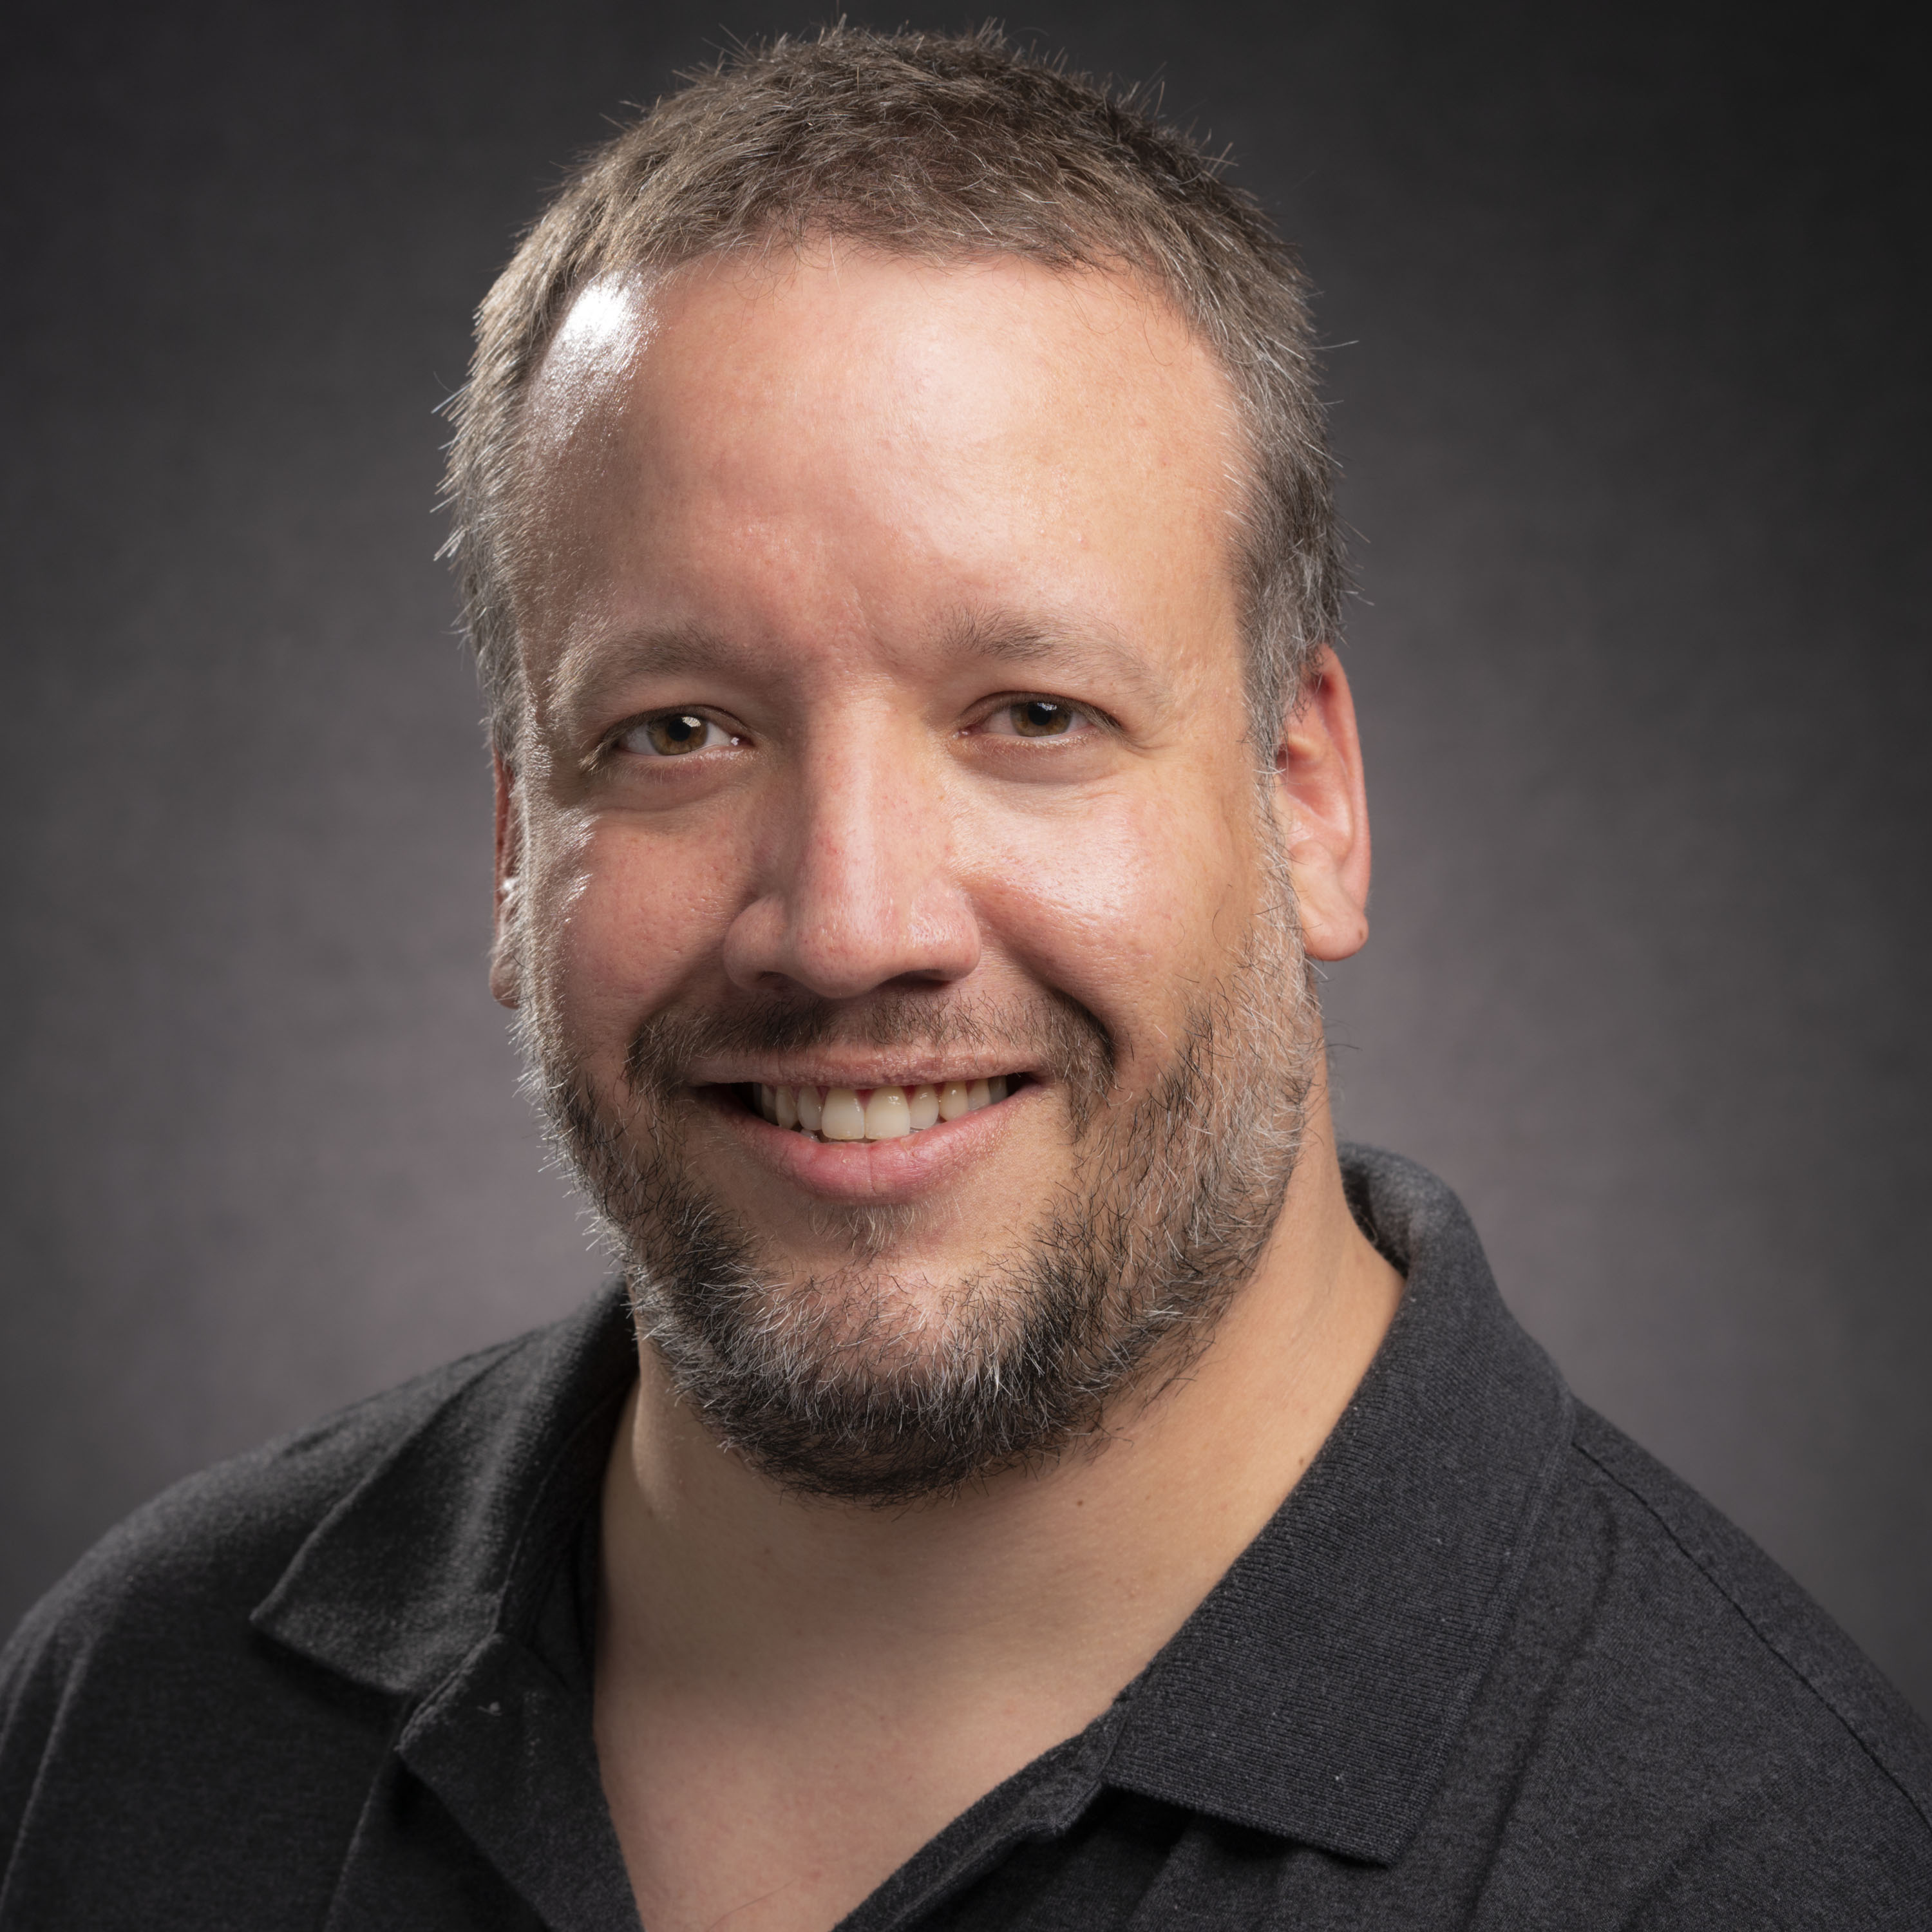
\includegraphics[width=0.4\linewidth]{jordan.jpg}
		\caption{Jordan Scott}
	\end{figure}

	\paragraph*{Contact Info: } jscott21@uccs.edu \\
	https://www.linkedin.com/in/jordan-cancer-scott/\\
	https://github.com/jordanmscott/uccs


	\paragraph*{About Me}
		
		
		
	I am just starting my PhD in Security program. My goal for this course is to get into a research frame of mind, learn the modern tricks and tips, and help refine my dissertation topic.
	
	
	I am really interested in learning more about zotero and latex. I gained some experience with zotero last year, but previously I've only been aware of manual tracking and editing. It's nice to know that technology has evolved quite a bit with research and data management.
	

	I have done stand-up comedy twice. My set was mostly cybersecurity related and I received a number of laughs. I'm not sure if my comedy career will continue, but my career will definitely be full of comedy. 
	

	
	
	
	\section{\textbf{Questions}}
	
	Question and Answers
	
	
	Question 1 - ?
	
	
	Answer 1 - ?

	
	Question 2 - ?
	
	
	Answer 2 - ?


	\section{\Merge Conflict Notes:}
	
	
	Not having access to the project seemed frustrating and took a bit to even figure out that was the problem. For my setup, I chose to use TeXstudio on a virtual box. The git clone part was easy. Getting the Assignment3 file to build was not. There were dependencies I needed to download/install into TeXstudio which was a challenge in itself, all related to the csvsimple function. Eventually got all that working. Then trying to figure out git itself... Got the commit part, the pull, the merge (had to install and configure a compare tool), and then the push. It's all working now and I definitely have a better understanding of git. The branches and stuff will get more interesting too. Anyways, I think I'm ready to start developing reports using this IDE/Git setup instead of manually transfering from overleaf.
		
	
%\end{document}

 